\chapter{Analisis Solusi}

\section{Arsitektur Solusi}

Setiap arsitektur solusi memiliki dua layanan eksternal, yaitu layanan pengguna dan layanan gerbang pembayaran. Kedua layanan ini akan dibuat \textit{stateless} sehingga penskalaan dapat dilakukan dengan menambah jumlah \textit{instance} layanan. Pada kasus ini, kedua layanan ini akan diusahakan sehingga tidak menjadi sumber \textit{bottleneck}. Layanan pengguna tidak akan menjadi \textit{bottleneck} karena pada saat pengujian akan diasumsikan seluruh pengguna sudah \textit{login} dan pemeriksaan otentikasi dilakukan pada masing-masing \textit{instance backend}.

Komunikasi dengan layanan pembayaran harus dilakukan secara sinkron, setidaknya ketika layanan tiket memanggil layanan pembayaran untuk membuat tagihan. Apabila layanan pembayaran tiket mengalami \textit{bottleneck} pada basis data, pengoptimalan pada basis data akan dilakukan dengan menggunakan kluster Citus sebagaimana yang dilakukan pada arsitektur yang mengoptimalkan PostgreSQL.

\subsection{Arsitektur Dasar Acuan (RADAR)}

RADAR akan menjadi dasar acuan yang digunakan sebagai dasar perbandingan kinerja. Arsitektur ini terdiri atas dua komponen, yaitu komponen layanan tiket dan kluster PostgreSQL. Kluster PostgreSQL ini terdiri atas satu \textit{leader} dan beberapa replika. Penggunaan replika bertujuan untuk meningkatkan \textit{throughput} pada operasi baca.

\begin{figure}[htbp]
    \centering
    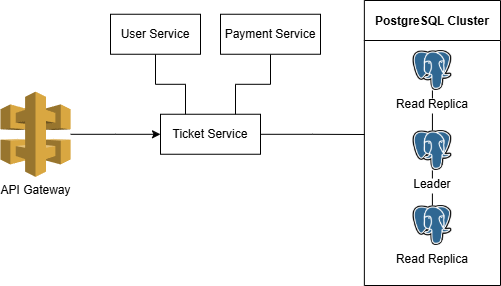
\includegraphics[width=0.8\textwidth]{resources/appendix/architecture-reference.png}
    \caption{Arsitektur Dasar Acuan}
    \label{fig:baseline-architecture}
\end{figure}

\subsubsection{Isu \textit{Replication Lag}}

Salah isu yang perlu diperhatikan pada arsitektur ini adalah \textit{replication lag}. Replika yang tertinggal selama beberapa detik pada kasus ini akan berdampak signifikan. Pada kasus ini, pendekatan solusinya akan bergantung pada keadaan yang dihadapi selama implementasi.

Pada proses pengujian, kluster PostgreSQL ini akan ditempatkan pada satu \textit{availability zone} yang sama, sehingga \textit{replication lag} tidak akan terjadi secara signifikan. Meskipun begitu, apabila terjadi \textit{replication lag} yang sangat besar, alternatif solusinya adalah dengan mengharuskan replika ACK terlebih dahulu sebelum penulisan dapat dilakukan, alih-alih melakukan replikasi secara asinkron.

\subsubsection{Penskalaan Pada RADAR}

Komponen \textit{backend} utama (layanan tiket) bersifat \textit{stateless}, sehingga dapat di-\textit{scale} dengan meningkatkan jumlah \textit{instance}. Kemudian, gerbang API akan melakukan \textit{load balancing} untuk mendistribusikan beban ke beberapa \textit{instance}.

Basis data merupakan komponen yang sulit di-\textit{scale} secara dinamis berdasarkan beban yang diterima. Biasanya, penskalaan secara vertikal merupakan opsi utama untuk meningkatkan \textit{throughput}, terutama dalam operasi tulis. Arsitektur ini membuat kluster PostgreSQL dengan konfigurasi satu node pemimpin dan sisanya node replika. Keberadaan replika memungkinkan peningkatan \textit{throughput} permintaan baca, meski tidak ada peningkatan \textit{throughput} untuk operasi tulis.

\subsubsection{Aspek Lain}

Pada saat penjualan, dapat diasumsikan entitas Events, TicketCategory, Areas, TicketSale, dan TicketPackage tidak berubah sehingga data entitas tersebut dapat di-\textit{cache}.

\subsection{Arsitektur yang Mengoptimalkan PostgreSQL (PGP)}

Arsitektur ini mengoptimalkan sistem dengan pola CQRS, pola penyeimbangan beban berbasiskan antrean, dan menggunakan ekstensi Citus untuk menjalankan basis data secara terdistribusi.

\begin{figure}[htbp]
    \centering
    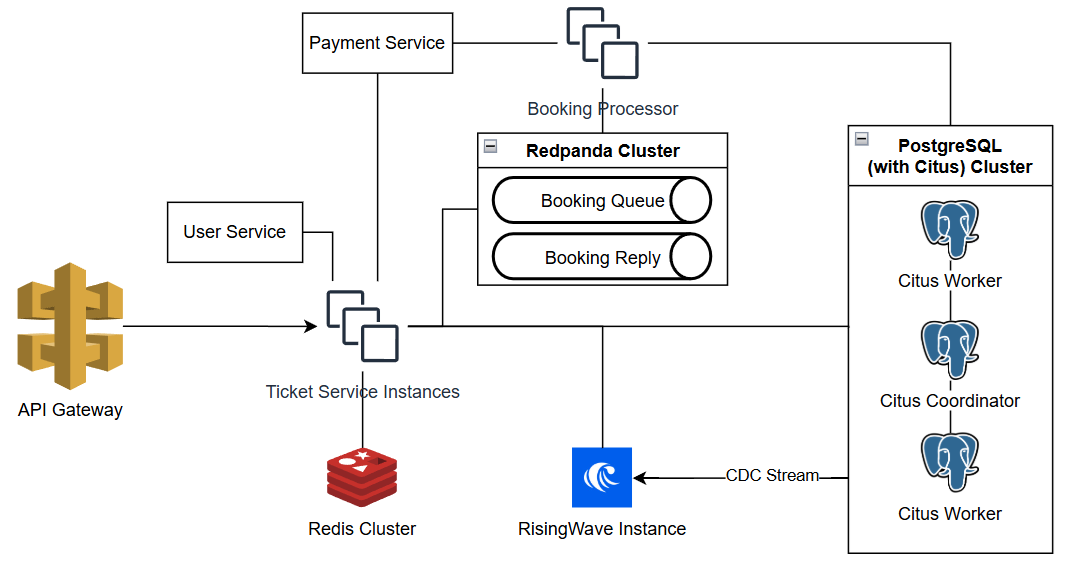
\includegraphics[width=1\textwidth]{resources/appendix/architecture-optimized.png}
    \caption{Arsitektur yang Mengoptimalkan PostgreSQL}
    \label{fig:optimized-architecture}
\end{figure}

\subsubsection{Peningkatan \textit{Throughput} PostgreSQL dengan Citus}

Penggunaan ekstensi Citus memungkinkan peningkatan \textit{throughput} dengan pendekatan \textit{scale-out}. Peningkatan ini tidak hanya pada \textit{throughput} baca, tetapi juga \textit{throughput} tulis. Hal ini dapat dicapai dengan pembagian data pada tabel berdasarkan baris, lalu setiap \textit{node} yang memegang bagian data tersebut dibuat menjadi \textit{writer}.

\textit{Sharding} berdasarkan baris dapat dilakukan pada tabel Seats, IssuedTicket, OrderItem, dan Orders. Entitas sisanya dapat dibuat sebagai tabel yang direplikasi ke setiap node.

\subsubsection{Penggunaan Pola Penyeimbangan Beban dengan Antrean}

Perintah pemesanan tiket (berupa \textit{command}/ \textit{event sourcing}) akan dimasukkan ke dalam antrean Redpanda terlebih dahulu. Lalu, \textit{booking processor} akan memproses permintaan secara bertahap berdasarkan kemampuan sistem. Pendekatan ini memungkinkan terjaganya stabilitas sistem ketika terdapat \textit{burst request}.

Selain itu, akan lebih baik apabila sistem dapat menolak permintaan pesanan lebih awal, seperti karena sudah ada pesanan yang sedang diproses tetapi masih belum \textit{commit}. Hal ini dapat didukung dengan penggunaan Redis untuk menyimpan \textit{uncommited data} yang akan digunakan untuk menolak permintaan pesanan lebih awal.

\begin{figure}[htbp]
    \centering
    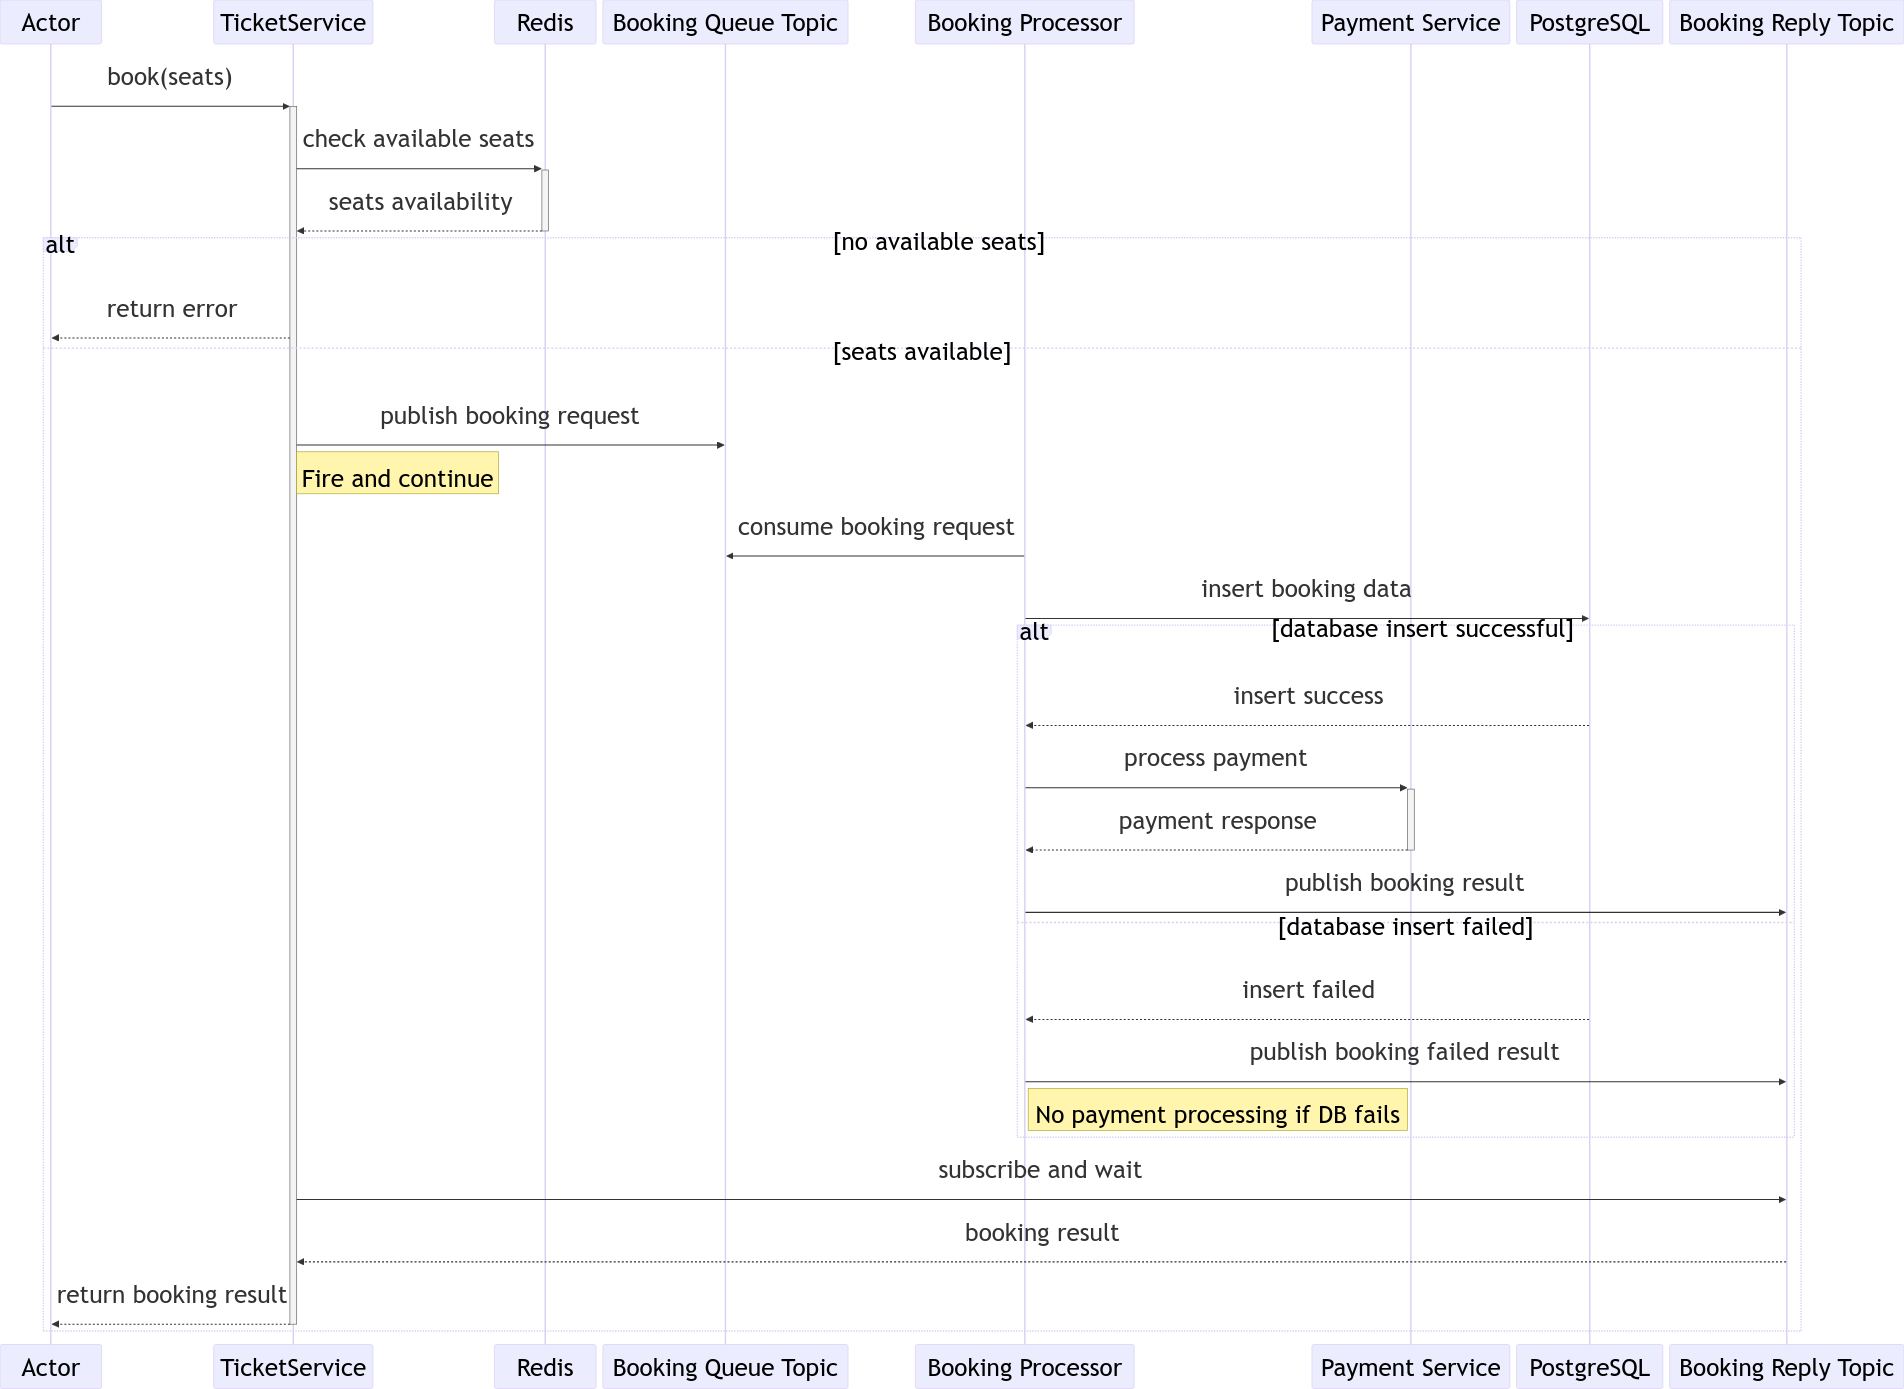
\includegraphics[width=1\textwidth]{resources/appendix/pgp-purchase-flow.png}
    \caption{Alur Pemesanan Tiket Pada PGP}
    \label{fig:pgp-purchase-flow}
\end{figure}

Terdapat dua isu yang harus dibahas pada pendekatan ini, yaitu:

\begin{enumerate}
    \item \textit{Persistence} pada Redis bersifat asinkron, sehingga terdapat kemungkinan data hilang ketika terjadi kegagalan. Meskipun begitu, penggunaan \textit{key-value store} lain yang \textit{persistent} berpotensi memperlambat kinerja. Dalam kasus ini, Redis akan dikonfigurasikan dalam mode kluster untuk penskalaan secara horizontal dan kombinasi antara \textit{snapshot} dan AOF untuk \textit{persistence}. Hilangnya data dapat terjadi ketika terdapat \textit{node} yang mengalami kegagalan. Meskipun begitu, \textit{data loss} atau \textit{eventual consistency} tidak akan mengganggu integritas sistem karena masih akan ada validasi lagi ketika pemrosesan pesanan.
    \item Isu \textit{fairness} harus diperhatikan ketika menggunakan Redpanda sebagai antrean. Redpanda hanya menjamin \textit{ordering} dalam satu partisi yang sama dan tidak menjamin \textit{ordering} secara global dalam satu topik. Salah satu cara untuk memastikan \textit{fairness} adalah dengan melakukan pembagian/ pemartisian antrean berdasarkan kategori tiket. Dengan begitu, pemrosesan pada antrean akan sesuai dengan urutan permintaan. Meskipun begitu, pendekatan ini mengharuskan pembelian lebih dari satu tiket dalam satu waktu hanya mendukung pemesanan dalam satu kategori yang sama.
    \item Dengan menggunakan antrean, komunikasi akan menjadi asinkron. Untuk menghubungkan permintaan dan respons, \textit{correlation id} dapat digunakan. Terdapat dua alternatif agar pengguna dapat diberitahu agar mendapatkan respons, yaitu menggunakan \textit{notify} dari sisi server atau respons pemesanan baru akan diberikan ketika sudah terdapat respons. Pendekatan yang dipilih adalah pendekatan kedua karena permintaan pemesanan juga membutuhkan aksi lanjutan untuk proses pembayaran. Selain itu, \textit{latency} pemrosesan permintaan ini juga dapat berguna sebagai \textit{metrics} dalam pengujian.
\end{enumerate}

\subsubsection{Pelimpahan Tanggung Jawab Baca Kepada RisingWave}

Pada permintaan baca ketersediaan tiket, tanggung jawab penanganannya dapat dilimpahkan kepada RisingWave. \textit{Streaming database} ini mengonsumsi \textit{CDC stream} dari kluster PostgreSQL, lalu memperbarui kueri secara inkremental. Dengan begitu, operasi baca tidak akan membebani basis data dan penanganannya dapat dilakukan dengan lebih efisien dengan RisingWave.

Sama seperti penggunaan \textit{read replica}, hal yang harus diperhatikan dalam penggunaan RisingWave adalah \textit{replication lag}. Data yang dikembalikan oleh RisingWave tidak valid apabila data tersebut \textit{outdated}. Pendekatan ini tidak mendukung konfigurasi agar transaksi \textit{commit} setelah RisingWave \textit{acknowledge} data, sehingga tetap akan ada \textit{replication lag}. Solusi dari permasalahan ini adalah \textit{tuning} RisingWave agar mampu mengikuti beban yang dikirimkan oleh PostgreSQL.

\subsubsection{Penskalaan Pada PGP}

Berikut adalah strategi penskalaan untuk setiap komponen selain dengan pendekatan \textit{scale-up}:

\begin{enumerate}
    \item Layanan tiket dapat di-\textit{scale} dengan menambah jumlah \textit{instance}.
    \item Redis dapat di-\textit{scale} dengan menggunakan konfigurasi kluster, sehingga data di-\textit{shard} berdasarkan \textit{range} hash. Penskalaan ini memungkinkan peningkatan \textit{throughput} untuk operasi baca dan tulis.
    \item Pemroses pesanan dapat di-\textit{scale} dengan menambah jumlah \textit{instance}. Jumlah pemroses ini mengikuti jumlah partisi pada topik.
    \item RisingWave dapat di-\textit{scale} dengan meningkatkan jumlah \textit{instance}. RisingWave dapat secara otomatis mengatur penggunaan sumber daya sehingga mampu menggunakan seluruh sumber daya yang tersedia.
    \item Kluster Redpanda dapat di-\textit{scale} dengan menggunakan beberapa partisi. Setiap partisi akan menangani permintaan untuk satu atau beberapa kategori tiket yang telah ditentukan. Jumlah partisi permintaan dan respons akan sama.
\end{enumerate}

\subsubsection{Aspek Lain}

\begin{enumerate}
    \item Pendekatan pemartisian berdasarkan kategori mengharuskan konfigurasi dilakukan secara manual setiap kali akan diadakan proses penjualan. Mekanisme atau analisis yang memungkinkan konfigurasi secara otomatis tidak akan dibahas karena di luar \textit{scope} penelitian ini.
    \item Penggunaan PostgreSQL dan kakas lain yang \textit{out of the box} memiliki banyak fitur memungkinkan \textit{extendability} yang lebih baik dengan kompleksitas yang tidak sebesar solusi EDA.
    \item Pada saat penjualan, dapat diasumsikan entitas Events, TicketCategory, Areas, TicketSale, dan TicketPackage tidak berubah sehingga data entitas tersebut dapat di-\textit{cache}.
\end{enumerate}

\subsubsection{Arsitektur \textit{Event-Driven} (EDA)}

Arsitektur ini tidak menggunakan PostgreSQL sama sekali. Pada dasarnya, basis data relasional terdiri atas komponen \textit{storage} dan \textit{query processor}. Pada arsitektur ini, komponen \textit{storage} diganti menggunakan Redpanda dengan berbagai topik dan \textit{query processor} diganti dengan RisingWave. Penggunaan RisingWave memungkinkan pembangunan kueri secara inkremental dari berbagai sumber data, termasuk topik Redpanda. Meskipun begitu, pendekatan ini tidak memiliki dukungan \textit{transaction} selain \textit{transaction} pada Redpanda yang berupa \textit{push log all or nothing} pada beberapa topik sekaligus. Untuk itu, Redis digunakan untuk menyimpan \textit{uncommited data} sehingga untuk mencegah \textit{double booking}.

\begin{figure}[htbp]
    \centering
    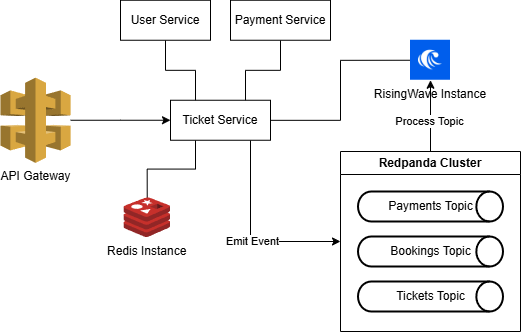
\includegraphics[width=1\textwidth]{resources/appendix/architecture-event-driven.png}
    \caption{Arsitektur EDA}
    \label{fig:solution-event-driven-architecture}
\end{figure}

\textbf{Pemodelan Topik dan Entitas}

Karena tidak ada basis data relasional yang digunakan dalam arsitektur ini, terdapat beberapa perubahan dalam pemodelan entitas menjadi topik. Perubahan ini adalah sebagai berikut:

\begin{enumerate}
    \item Topik Events merupakan hasil denormalisasi entitas Tickets, TicketCategory, dan Areas.
    \item Topik Seats merupakan entitas Seats. Topik ini juga menyimpan \textit{log} perubahan status \textit{seat}. Contoh: Seat-A-Available, Seat-A-Pending.
    \item Topik TicketSales merupakan hasil denormalisasi entitas TicketSale dan TicketPackage.
    \item Topik Orders merupakan hasil denormalisasi entitas Orders, OrderItem. Topik ini juga menyimpan \textit{log} perubahan status Order.
    \item Topik IssuedTickets merupakan entitas IssuedTicket.
\end{enumerate}

\textbf{Alur Sistem}

Berikut adalah gambaran alur sistem untuk proses pemesanan tiket dan notifikasi pembayaran.

\begin{figure}[htbp]
    \centering
    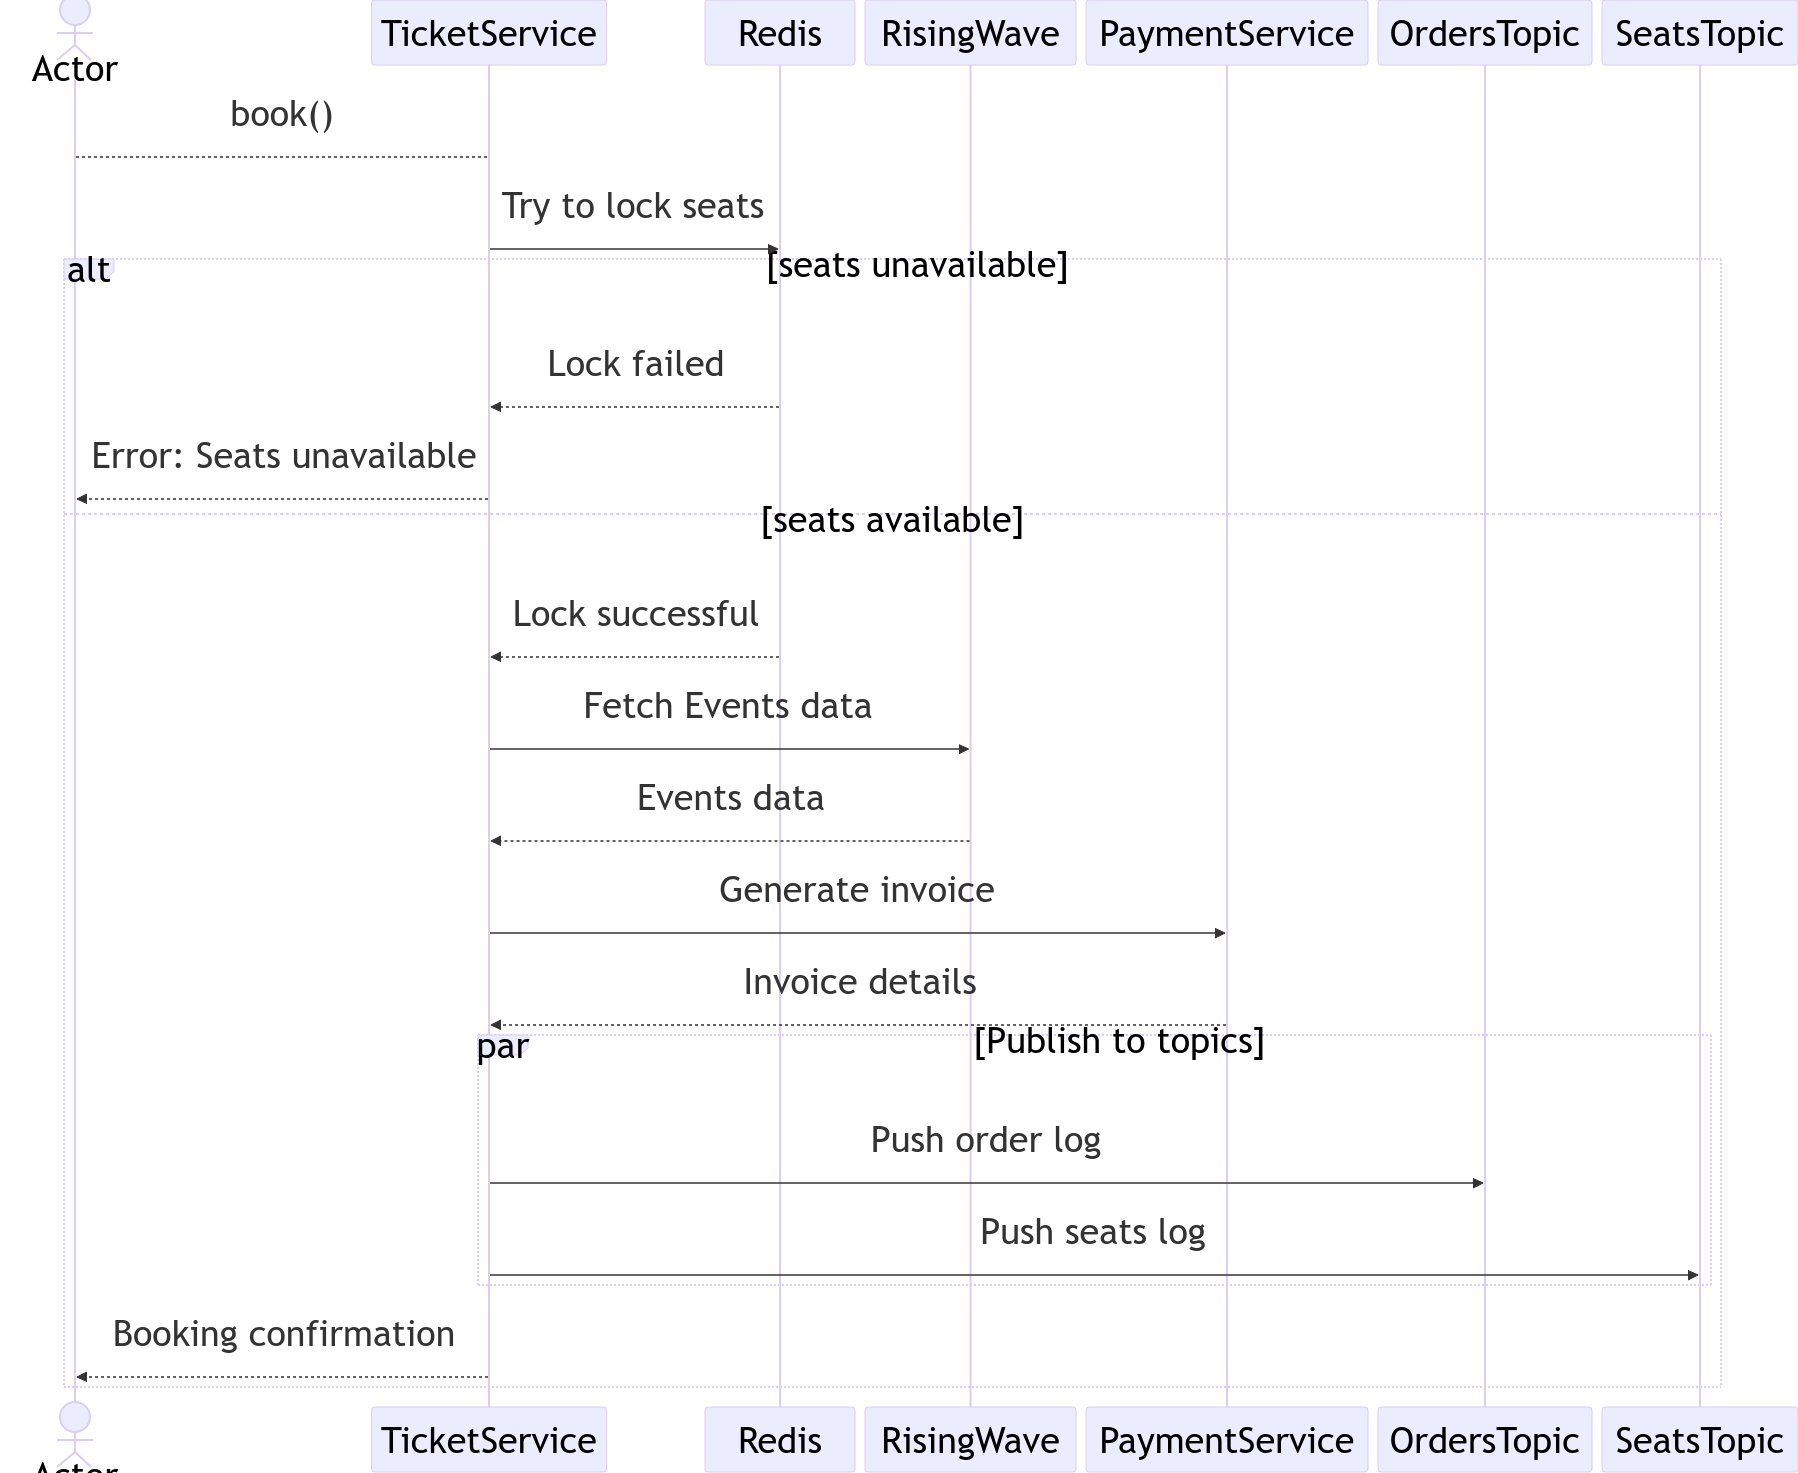
\includegraphics[width=1\textwidth]{resources/appendix/eda-book.png}
    \caption{Alur Pemesanan Tiket pada Arsitektur EDA}
    \label{fig:book-flow-eda}
\end{figure}

\begin{figure}[htbp]
    \centering
    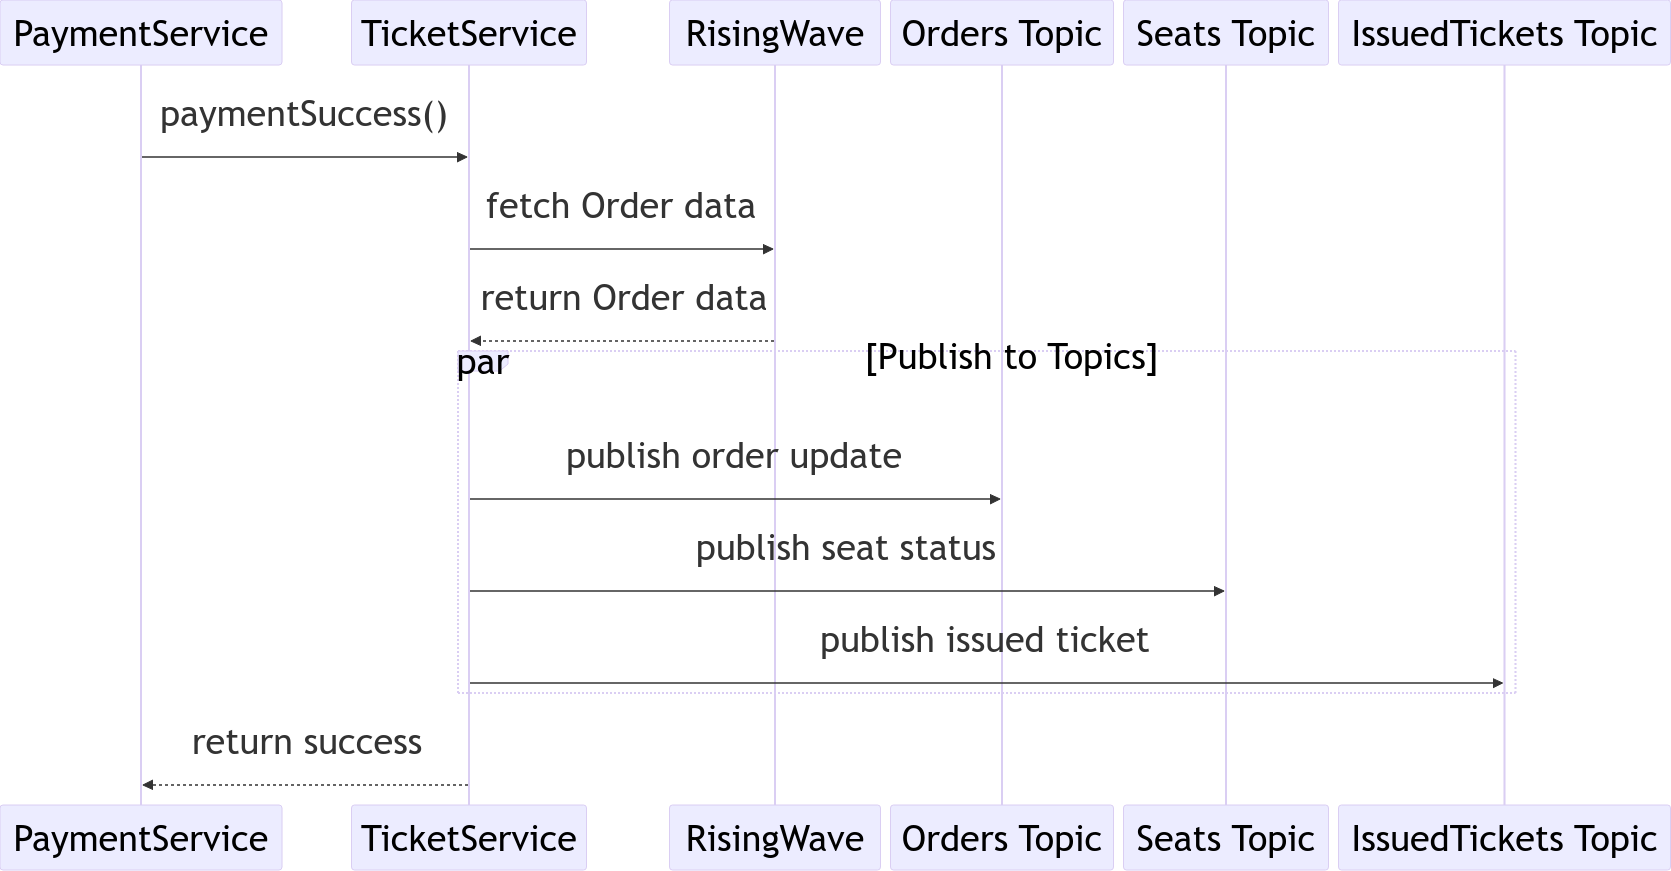
\includegraphics[width=1\textwidth]{resources/appendix/eda-verify-payment.png}
    \caption{Alur Verifikasi Pembayaran pada Arsitektur EDA}
    \label{fig:payment-verify-flow-eda}
\end{figure}

\textbf{Penskalaan Arsitektur EDA}

Berikut adalah strategi penskalaan untuk setiap komponen selain dengan pendekatan \textit{scale-up}:

\begin{enumerate}
    \item Layanan tiket dapat di-\textit{scale} dengan menambah jumlah \textit{instance}.
    \item Redis dapat di-\textit{scale} dengan menggunakan konfigurasi kluster, sehingga data di-\textit{shard} berdasarkan \textit{range} hash. Penskalaan ini memungkinkan peningkatan \textit{throughput} untuk operasi baca dan tulis.
    \item  RisingWave dapat di-\textit{scale} dengan meningkatkan jumlah \textit{instance}. RisingWave dapat secara otomatis mengatur penggunaan sumber daya sehingga mampu menggunakan seluruh sumber daya yang tersedia.
    \item Kluster Redpanda dapat di-\textit{scale} dengan menggunakan beberapa partisi.
\end{enumerate}

\textbf{Isu \textit{Persistence} Pada \textit{Uncommited Data}}

Arsitektur ini membutuhkan \textit{persistence} yang lebih kuat dibandingkan dengan arsitektur sebelumnya. Meskipun begitu, penggunaan \textit{snapshot}, AOF, dan konfigurasi \texttt{appendfsync always} dapat dianggap cukup. Perintah \texttt{appendfsync always} membuat Redis untuk selalu melakukan penulisan langsung setelah setiap perintah penulisan dijalankan. Hal ini berbeda dengan konfigurasi \textit{default} Redis yang melakukan operasi tulis setiap detik. Meskipun begitu, penggunaan konfigurasi ini menjadikan \textit{throughput} tulis Redis jauh lebih lambat. Akan tetapi, hal ini menjadi risiko yang diambil untuk menjamin \textit{safety} pada sistem ini.

\textbf{Aspek Lain}

\begin{enumerate}
    \item Dibandingkan dengan arsitektur sebelumnya, pendekatan seperti ini memiliki kompleksitas yang jauh lebih tinggi. Selain itu, aspek \textit{extendability} pada arsitektur ini tidak lebih baik dibandingkan dengan arsitektur sebelumnya, terutama pada penambahan fitur yang berinteraksi dengan basis data relasional.
    \item Pada saat penjualan, dapat diasumsikan entitas Events, TicketCategory, Areas, TicketSale, dan TicketPackage tidak berubah sehingga data entitas tersebut dapat di-\textit{cache}.
    \item Redis merupakan basis data yang menyimpan data di memori. \textit{Data eviction} tidak boleh terjadi ketika menggunakan Redis pada arsitektur ini, sehingga alokasi memori Redis merupakan hal yang perlu perhatian khusus dan harus dijamin agar tidak mengalami \textit{out of memory}.
\end{enumerate}




\section{Alternatif Solusi}

Bagian ini membahas alternatif pengoptimalan atau alternatif teknologi yang bisa menjadi opsi, tetapi tidak dipilih menjadi bagian dari solusi.

\section{Penggunaan \textit{Cache} dengan TTL Kecil}

Meski pada beban tinggi hasil kueri yang di-\textit{cache} akan selalu \textit{stale}, tetap ada durasi hidup (\textit{time to live}) \textit{cache} yang masih dapat diterima. Misalkan, waktu hidup \textit{cache} pembacaan ketersediaan adalah 100-200 milidetik. Rentang waktu ini masih memberikan \textit{data freshness} yang baik dan mampu meminimalkan jumlah kueri yang harus dilakukan sistem. Meskipun begitu, pendekatan ini harus dilakukan pada setiap arsitektur agar perbandingannya setara. Selain itu, pendekatan ini tidak sesuai dengan tujuan tugas akhir ini yang ingin mengoptimalkan operasi baca dan tetap memberikan hasil kueri yang \textit{fresh}.

\section{Alternatif Basis Data Terdistribusi}

Selain Citus, terdapat berbagai alternatif basis data terdistribusi lain, seperti Vitess, TiDB, YugabyteDB, dan CockroachDB. Berikut adalah perbandingan masing-masing solusi \parencite{citus,vitess,tiDB,yugabyte,cockroachDB}:

\begingroup
\footnotesize
\begin{longtable}{|p{0.14\textwidth}|p{0.14\textwidth}|p{0.14\textwidth}|p{0.14\textwidth}|p{0.14\textwidth}|p{0.14\textwidth}|}
    \caption{Perbandingan Antara Citus, Vitess, TiDB, YugabyteDB, dan CockroachDB}                                                                                                                                                                                                                    \\
    \hline
    \textbf{Aspek}            & \textbf{Citus}                                               & \textbf{Vitess}                                     & \textbf{TiDB}                                  & \textbf{YugabyteDB}                            & \textbf{CockroachDB}                           \\
    \hline
    \endfirsthead

    \multicolumn{6}{|c|}{\tablename\ \thetable\ -- \textit{Lanjutan dari halaman sebelumnya}}                                                                                                                                                                                                         \\
    \hline
    \textbf{Aspek}            & \textbf{Citus}                                               & \textbf{Vitess}                                     & \textbf{TiDB}                                  & \textbf{YugabyteDB}                            & \textbf{CockroachDB}                           \\
    \hline
    \endhead

    \hline
    \multicolumn{6}{|r|}{\textit{Dilanjutkan ke halaman berikutnya}}                                                                                                                                                                                                                                  \\
    \endfoot

    \hline
    \endlastfoot

    \hline
    Basis data yang mendasari & PostgreSQL                                                   & MySQL                                               & Dibuat dari awal                               & Dibuat dari awal                               & Dibuat dari awal                               \\
    \hline
    \hline
    Arsitektur                & \textit{Sharded Multi-Master with a Coordinator}             & \textit{Sharded Multi-Master with a Coordinator}    & \textit{Multi-Master with Shared Nothing}      & \textit{Multi-Master with Shared Nothing}      & \textit{Multi-Master with Shared Nothing}      \\
    \hline
    \hline
    Tipe                      & Ekstensi PostgreSQL                                          & Ekstensi MySQL                                      & Basis data terdistribusi dengan konsensus Raft & Basis data terdistribusi dengan konsensus Raft & Basis data terdistribusi dengan konsensus Raft \\
    \hline
    \hline
    Kompatibilitas SQL        & PostgreSQL                                                   & MySQL                                               & Kompatibel dengan MySQL 8.0                    & Kompatibel dengan PostgreSQL                   & Kompatibel dengan PostgreSQL                   \\
    \hline
    \hline
    Konsistensi               & Sama seperti PostgreSQL (konsisten dalam satu \textit{node}) & \textit{Eventual consistent} untuk operasi tertentu & ACID                                           & ACID                                           & ACID                                           \\
    \hline
    \hline
    Dukungan CDC              & Ada                                                          & Ada                                                 & Ada                                            & Ada                                            & Ada                                            \\
    \hline
    \hline
    Distribusi Data           & \textit{shard}                                               & \textit{shard}                                      & \textit{native distributed}                    & \textit{native distributed}                    & \textit{native distributed}                    \\
    \hline
\end{longtable}
\endgroup

Distribusi data yang \textit{natively distributed} masih sama-sama berupa \textit{sharding} data. Meskipun begitu, proses \textit{sharding} ini dilakukan secara otomatis dan tidak ditentukan oleh pengguna. Selain itu, suatu \textit{shard} dapat dipegang oleh beberapa \textit{node} sekaligus untuk mencapai \textit{redundancy} dan \textit{fault tolerance}.

Pada basis data terdistribusi seperti YugabyteDB, CockroachDB, dan TiDB, terdapat \textit{overhead} dalam koordinasi antarnode untuk operasi tulis, terlebih lagi setiap operasi tulis harus mencapai konsensus terlebih dahulu. Berbeda dengan basis data terdistribusi yang memakai koordinator seperti Citus dan Vitess, \textit{overhead} lebih kecil dan berada pada koordinator saja. Setelah koordinator menentukan node yang bertanggung jawab atas operasi tersebut, operasi langsung diarahkan kepada node yang berkaitan. Pendekatan konsensus memang memberikan konsistensi dan \textit{failover} yang lebih baik, tetapi terdapat \textit{tradeoff} berupa latensi yang lebih tinggi. Penggunaan basis data terdistribusi dengan konsensus akan lebih \textit{desirable} apabila melayani pengguna dalam beberapa \textit{region} yang berbeda. Meskipun begitu, penelitian ini berfokus pada pengoptimalan untuk satu \textit{region} yang sama.

Berdasarkan pembahasan di atas, terdapat dua pilihan yang tersisa, yaitu Vitess dan Citus. Citus dipilih agar basis \textit{database} yang digunakan sama, sehingga perbandingan antar arsitektur lebih disebabkan karena perbedaan arsitektur dan bukan karena perbedaan pengoptimalan pada basis data yang berbeda. Selain itu, basis data PostgreSQL merupakan basis data yang paling familiar dengan penulis dibandingan dengan MySQL.


\subsection{Penggunaan Solusi Basis Data \textit{Serverless}}

Penggunaan solusi serverless seperti Supabase, Neon, dan PlanetScale terbatas pada vendor tersebut. Solusi seperti ini memiliki banyak variabel yang tidak bisa dikontrol, terlebih lagi dari aspek biaya yang harus dikeluarkan untuk melakukan pengujian. Selain itu, terdapat batas atas penggunaan sumber daya yang diperbolehkan oleh setiap vendor. Batas atas ini baru bisa ditambah ketika melakukan \textit{subscription} dengan \textit{enterprise plan}. Oleh karena itu, penggunaan solusi \textit{serverless} tidak \textit{feasible} untuk dilakukan.

\section{Penggunaan Redpanda dan Alternatifnya}

Arsitektur perpesanan bisa dibagi menjadi dua, yaitu \textit{brokered} dan \textit{brokerless}. Arsitektur \textit{brokerless} menawarkan latensi yang lebih rendah dan \textit{deployment} yang lebih sederhana, tetapi tidak memiliki fitur seperti \textit{message durability}, \textit{partitioning}, dan \textit{replayability}. Oleh karena itu, ide solusi dengan antrean dan \textit{storage} untuk arsitektur \textit{event-driven} akan menggunakan arsitektur \textit{brokered}.

Model \textit{message broker} yang saling berbeda setidaknya saat ini dapat direpresentasikan oleh Apache Kafka, RabbitMQ, dan NATS. Berikut adalah perbandingan umum dari ketiga \textit{broker} tersebut \parencite{arshadChoosingTheRightMessaging,royNatsRmqKafka,studyOnModeryMessaging}:

\begingroup
\footnotesize
\begin{longtable}{|p{0.14\textwidth}|p{0.24\textwidth}|p{0.24\textwidth}|p{0.24\textwidth}|}
    \caption{Perbandingan Antara Kafka, RabbitMQ, dan NATS}                                                                                                                                                                    \\
    \hline
    \textbf{Aspek}               & \textbf{Kafka}                                                       & \textbf{RabbitMQ}                             & \textbf{NATS}                                                        \\
    \hline
    \endfirsthead

    \multicolumn{4}{|c|}{\tablename\ \thetable\ -- \textit{Lanjutan dari halaman sebelumnya}}                                                                                                                                  \\
    \hline
    \textbf{Aspek}               & \textbf{Kafka}                                                       & \textbf{RabbitMQ}                             & \textbf{NATS}                                                        \\
    \hline
    \endhead

    \hline
    \multicolumn{4}{|r|}{\textit{Dilanjutkan ke halaman berikutnya}}                                                                                                                                                           \\
    \endfoot

    \hline
    \endlastfoot

    \hline
    Ditulis dalam                & Scala, Java                                                          & Erlang                                        & Go                                                                   \\
    \hline
    Model Penyimpanan            & \textit{Log-based}                                                   & \textit{Queue-based}                          & \textit{Log-based}, \textit{Transient} (\textit{in-memory})          \\
    \hline
    \textit{Message Persistence} & \textit{Persistent}                                                  & \textit{Persistent} dan \textit{ephemeral}    & \textit{Persistent} dan \textit{ephemeral}                           \\
    \hline
    \textit{Throughput}          & Hingga 2 juta pesan per detik                                        & Hingga 60 ribu pesan per detik                & Hingga 6 juta pesan per detik                                        \\
    \hline
    Latensi                      & \textit{Low ms}                                                      & \textit{Low ms}                               & \textit{Sub-ms}                                                      \\
    \hline
    Model penskalaan             & Horizontal (dengan partisi)                                          & Terbatas                                      & Horizontal (mode kluster)                                            \\
    \hline
    Model Topik                  & Topik terpartisi                                                     & \textit{Queues}                               & \textit{Subject-based Topics}                                        \\
    \hline
    Model Konsumen               & \textit{Pull-based}                                                  & \textit{Push-based}                           & \textit{Pull or push-based}                                          \\
    \hline
    Protokol yang Didukung       & Kafka                                                                & AMQP, MQTT, STOMP                             & NATS, MQTT                                                           \\
    \hline
    \textit{Ordering Guarantee}  & Level partisi                                                        & Level \textit{queue}                          & Per subjek                                                           \\
    \hline
    \textit{Replayability}       & Ya                                                                   & Tidak                                         & Ya                                                                   \\
    \hline
    Penghapusan Pesan            & Tidak. Disimpan berdasarkan \textit{retention policy}                & Ya. Dihapus setelah pemrosesan                & Dapat diatur                                                         \\
    \hline
    \textit{Delivery Guarantee}  & \textit{At most once}, \textit{at least once}, \textit{exactly once} & \textit{At most once}, \textit{at least once} & \textit{At most once}, \textit{at least once}, \textit{exactly once} \\
    \hline
\end{longtable}
\endgroup

Solusi \textit{queue} dan solusi \textit{event-driven} membutuhkan \textit{messaging platform} yang memiliki semantik \textit{exactly once} dengan \textit{throughput} tinggi. Selain itu, solusi \textit{event-driven} juga membutuhkan \textit{persistence} dan \textit{durability}. Pilihan yang tersedia adalah Apache Kafka dan NATS. RabbitMQ tidak dipilih karena memiliki masalah pada \textit{throughput} dan tidak menawarkan \textit{durability} dan \textit{replayability}. Pada akhirnya, Apache Kafka merupakan \textit{platform} yang dipilih. Meskipun NATS juga mampu memenuhi kebutuhan, fitur-fitur tersebut merupakan fitur tambahan yang bukan menjadi tujuan awal dari pembuatan NATS dan tergolong masih baru.

Meskipun begitu, Apache Kafka memiliki masalah pada efisiensi sumber daya dan sulit dikelola. Oleh karena itu, terdapat alternatif \textit{messaging platform} yang Kafka-\textit{compatible} seperti Redpanda. Redpanda memiliki latensi yang lebih rendah, pengoptimalan yang lebih baik, dan lebih mudah untuk dikelola dibandingkan dengan Kafka \parencite{comparingKafkaAlternatives}. Oleh karena itu, Redpanda menjadi pilihan yang lebih layak dibandingkan dengan kafka.

\subsection{Penggunaan RisingWave dan Alternatifnya}

Bahas butuh exactly once semantics. Evaluate opsi yang ada

Flink, RisingWave, Apache Kafka Stream (or Redpanda)

Bahas kenapa RisingWave
- kinerja (Rust, NonJVM)
- Integrasi langsung dengan CDC Postgres, Kafka

\subsection{Penggunaan Redis dan Alternatifnya}

Kenapa Redis dibandingkan dengan solusi KV lain

local dengan replikasi (redis), consensus based,

Konsensus: etcd, TiKV
Persistent: LevelDB by Google, RocksDB (fork of LevelDB by Facebook)
Fork redis: Valkey
